\documentclass[10pt,a4paper]{amsart}
\usepackage[margin=19mm]{geometry}
\usepackage{amsmath,amssymb,mathtools}
\usepackage[scr=rsfs,cal=euler]{mathalfa}
\usepackage{xfrac}
\usepackage[unicode,hidelinks,bookmarks=false]{hyperref}
\newcommand{\ie}{i.e.\ }
\newcommand{\cf}{cf.\ }
\newcommand{\resp}{respectively\ }
\newcommand{\Subsection}{\subsection}
\providecommand{\nobreakdash}{\nobreak\hbox{-}}
\setlength{\emergencystretch}{2em}
\multlinegap0pt
\usepackage{tikz}
\usepackage{amssymb}
\usepackage{float}
\usepackage[normalem]{ulem}
\usepackage{caption}
\newtheorem{lem}{Lemma}
\title{Entropy bounds, Compactness and Finiteness Theorems for Embedded self-shrinkers with rotational symmetry}
\author{John Man Shun Ma, Ali Muhammad, Niels Martin M\o ller}
\date{Source: arXiv:2202.08641v2 (CC BY 4.0)}
\begin{document}
\maketitle

\noindent\emph{Source and licence.} Entropy bounds, Compactness and Finiteness Theorems for Embedded self-shrinkers with rotational symmetry. Version arXiv:2202.08641v2 (CC BY 4.0), distributed by arXiv under the Creative Commons Attribution 4.0 International licence, http://creativecommons.org/licenses/by/4.0/, as recorded in the arXiv licence metadata for this exact version and shown on the abstract page https://arxiv.org/abs/2202.08641v2. Full licence notice: \texttt{licenses/arxiv-2202.08641-CC-BY-4.0.txt}.\par\smallskip

\noindent\textit{Editorial scope.} Counted unit: the article's lem 3 (source0.tex lines 619--621). The article's complete original proof of it is delivered with it (source0.tex lines 623--764, one \texttt{proof} environment of 142 lines). No mathematics is written, repaired or re-derived: the statement and the proof are the article's own lines, in the article's own notation, and no retained line is substituted or re-flowed.  Retained uncounted as the source-local context the proof needs: lines 436--437; lines 605--611.  Nothing was omitted from any retained span, so the package carries no omission record.  No retained line contains a citation, so the wrapper carries no bibliography and no bibliography entry.  The retained lines contain the article's own diagram code, which the wrapper typesets with the standard tikz packages; no image file is delivered and the package declares no asset dependency.  Editorial formatting only, in addition: an AMS \texttt{amsart} preamble that restates the article's own declarations and macros used by the retained lines, namely the environments \texttt{lem} on separate counters, together with the standard packages those lines need.  The retained environments print in this document as Lemma 1 in order of appearance, whereas the article prints the same items with the numbering of its own full document.  The complete native source of the article as distributed in the arXiv e-print for this exact version is bundled unchanged as \texttt{sources/122201/source0.tex}.
		\begin{lem} \label{claim 1} There is $R_1 \ge R_0$ so that the following holds: for all $R \ge R_1$, there is $k_1 = k_1(R)$ so that for all $k\ge k_1$, $\operatorname{Im}\sigma_k\cap K_R$ contains a connected component different from $\sigma_k (I_{k,R})$ which intersects $K_{R_1}$. 
		\end{lem}

		\begin{lem} \label{sigma^c_k stays close to sigma_infty}
			By passing to a subsequence of $(\sigma_k)$ if necessary,  
			\begin{equation} \label{eqn sigma^C_k closed to sigma_infty}
				|\sqrt{x^2+r^2} - \sqrt{2n}|<R_k^{-1}
			\end{equation}
			for all $(x, r)\in \operatorname{Im} (\sigma_k) \cap K_{R_k}$ and for all $k\in \mathbb N$.
		\end{lem}

		\begin{lem} \label{claim 3} 
			The sequence of self-shrinkers $(\Sigma_{\sigma_k})_{k=1}^\infty$ converges in Hausdorff distance to the round sphere $\Sigma_{\sigma_\infty}$ as $k\to \infty$. 
		\end{lem}

		\begin{proof} [Proof of Lemma \ref{claim 3}] We use a maximum principle argument similar to that in the proof of Lemma \ref{claim 1}. Let $\epsilon>0$. Let $t_0 \in (-1, 0)$ be given by 
			\begin{equation} \label{eqn choice of t_0}
				\sqrt{-t_0} = \frac{\sqrt{2n} + 0.5\epsilon}{\sqrt{2n}+\epsilon}.
			\end{equation}
			Let $k_\epsilon \in \mathbb N$ be large such that $R_{k_\epsilon}^{-1}<\epsilon/2$ and the following holds: there are two horizontal translations and scalings of the Angenent torus $\Sigma_{\bar a_\pm}$ so that
			
			\begin{itemize}
				\item the image of $\bar a_+$ and $\bar a_-$ lie in $K_{R_{k_\epsilon}}$, 
				\item $\sqrt{2n}+R_{k_\epsilon}^{-1}< \sqrt{x^2+r^2} <\sqrt{2n}+\epsilon$ for all $(x, r) \in \operatorname{Im} \bar a_+$, 
				\item $\sqrt{2n}-\epsilon <\sqrt{x^2+r^2}<\sqrt{2n}-R_{k_\epsilon}^{-1}$ for all $(x, r) \in \operatorname{Im} \bar a_-$, and
				\item the MCF starting at $\Sigma_{\bar a_\pm}$ at $t=-1$ shrinks to $(\sqrt{2n} \pm 0.5\epsilon, 0)$ at time $t_e <t_0$. 
			\end{itemize}
			By Lemma \ref{sigma^c_k stays close to sigma_infty}, $\bar a_{\pm}$ do not intersect with $\sigma_k$ when $k\ge k_\epsilon$.
			\begin{figure}[ht]
				\tikzset{every picture/.style={line width=0.75pt}} %set default line width to 0.75pt        
				
				\begin{tikzpicture}[x=0.75pt,y=0.75pt,yscale=-1,xscale=1]
					%uncomment if require: \path (0,196); %set diagram left start at 0, and has height of 196
					
					%Straight Lines [id:da9926041072992973] 
					\draw  [dash pattern={on 4.5pt off 4.5pt}]  (124,161) -- (498.8,160.01) ;
					\draw [shift={(500.8,160)}, rotate = 179.85] [color={rgb, 255:red, 0; green, 0; blue, 0 }  ][line width=0.75]    (10.93,-3.29) .. controls (6.95,-1.4) and (3.31,-0.3) .. (0,0) .. controls (3.31,0.3) and (6.95,1.4) .. (10.93,3.29)   ;
					%Curve Lines [id:da7124915754112757] 
					\draw [color={rgb, 255:red, 155; green, 155; blue, 155 }  ,draw opacity=0.52 ] [dash pattern={on 4.5pt off 4.5pt}]  (290.8,3) .. controls (306.8,55) and (313.8,103) .. (313.19,160.5) ;
					%Curve Lines [id:da6063775145528378] 
					\draw [color={rgb, 255:red, 245; green, 166; blue, 35 }  ,draw opacity=1 ] [dash pattern={on 4.5pt off 4.5pt}]  (147.8,3) .. controls (159.8,39) and (164.8,115) .. (163.4,159.5) ;
					%Straight Lines [id:da1921120594778276] 
					\draw [color={rgb, 255:red, 35; green, 211; blue, 33 }  ,draw opacity=1 ] [dash pattern={on 4.5pt off 4.5pt}]  (125,143) -- (495.8,143) ;
					%Curve Lines [id:da7201937522241064] 
					\draw [color={rgb, 255:red, 35; green, 211; blue, 33 }  ,draw opacity=1 ] [dash pattern={on 4.5pt off 4.5pt}]  (270.8,3) .. controls (288.8,37) and (296.8,89) .. (297.01,159.22) ;
					%Shape: Polygon Curved [id:ds4450714038175556] 
					\draw  [color={rgb, 255:red, 208; green, 2; blue, 2 }  ,draw opacity=1 ][line width=1.5]  (382.4,121.8) .. controls (382.4,115.81) and (385.52,110) .. (392.74,110) .. controls (399.96,110) and (403.86,114.72) .. (403.86,121.8) .. controls (403.86,128.88) and (399.37,136.87) .. (392.93,136.87) .. controls (386.5,136.87) and (382.4,127.79) .. (382.4,121.8) -- cycle ;
					%Shape: Polygon Curved [id:ds2697272844122598] 
					\draw  [color={rgb, 255:red, 208; green, 2; blue, 2 }  ,draw opacity=1 ][line width=1.5]  (222.4,119.8) .. controls (222.4,113.81) and (225.52,108) .. (232.74,108) .. controls (239.96,108) and (243.86,112.72) .. (243.86,119.8) .. controls (243.86,126.88) and (239.37,134.87) .. (232.93,134.87) .. controls (226.5,134.87) and (222.4,125.79) .. (222.4,119.8) -- cycle ;
					%Curve Lines [id:da5546905209743642] 
					\draw [color={rgb, 255:red, 35; green, 211; blue, 33 }  ,draw opacity=1 ] [dash pattern={on 4.5pt off 4.5pt}]  (310.8,4) .. controls (321.8,50) and (330.8,100) .. (331.01,161.22) ;
					%Curve Lines [id:da9706183349305664] 
					\draw [color={rgb, 255:red, 245; green, 166; blue, 35 }  ,draw opacity=1 ] [dash pattern={on 4.5pt off 4.5pt}]  (450.8,2) .. controls (462.8,38) and (467.8,114) .. (466.4,158.5) ;
					
					% Text Node
					\draw (320.4,164.9) node [anchor=north west][inner sep=0.75pt]  [font=\scriptsize,color={rgb, 255:red, 126; green, 211; blue, 33 }  ,opacity=1 ]  {$\sqrt{2n} +R_{k_{\epsilon }}^{-1}$};
					% Text Node
					\draw (243.4,164.4) node [anchor=north west][inner sep=0.75pt]  [font=\scriptsize,color={rgb, 255:red, 126; green, 211; blue, 33 }  ,opacity=1 ]  {$\sqrt{2n} -R_{k_{\epsilon }}^{-1}$};
					% Text Node
					\draw (139.4,167.4) node [anchor=north west][inner sep=0.75pt]  [font=\scriptsize,color={rgb, 255:red, 245; green, 166; blue, 35 }  ,opacity=1 ]  {$\sqrt{2n} -\epsilon $};
					% Text Node
					\draw (441.4,165.4) node [anchor=north west][inner sep=0.75pt]  [font=\scriptsize,color={rgb, 255:red, 245; green, 166; blue, 35 }  ,opacity=1 ]  {$\sqrt{2n} +\epsilon $};
					% Text Node
					\draw (504,151.4) node [anchor=north west][inner sep=0.75pt]    {$x$};
					% Text Node
					\draw (497,130.4) node [anchor=north west][inner sep=0.75pt]  [color={rgb, 255:red, 33; green, 211; blue, 65 }  ,opacity=1 ]  {$r=R_{k_{\epsilon }}^{-1}$};
					% Text Node
					\draw (388,89.4) node [anchor=north west][inner sep=0.75pt]  [color={rgb, 255:red, 208; green, 13; blue, 2 }  ,opacity=1 ]  {$\overline{a}_{+}$};
					% Text Node
					\draw (230,87.4) node [anchor=north west][inner sep=0.75pt]  [color={rgb, 255:red, 208; green, 2; blue, 2 }  ,opacity=1 ]  {$\overline{a}_{-}$};
					
					
				\end{tikzpicture}
				\caption{Choices of $\bar a_\pm$.}
			\end{figure}
			
			Now we claim that 
			\begin{align} \label{Hausdorff converges to round sphere eqn}
				\sqrt{2n}-\epsilon<\sqrt{x^2+r^2}<\sqrt{2n}+\epsilon, \ \ \text{ for all }(x,r)\in \operatorname{Im}\sigma_k, \ k\ge k_\epsilon.
			\end{align}
			By Lemma \ref{sigma^c_k stays close to sigma_infty} and that $R_{k_\epsilon}^{-1}<\epsilon$, it suffices to consider points outside $K_{R_{k_\epsilon}}$. Fix any $k\ge k_\epsilon$. If there is $(x,r)\in \operatorname{Im}(\sigma_k)$ so that $\sqrt{x^2+r^2} \ge \sqrt{2n} +\epsilon$, then since each $\sigma_k$ is connected, there is a subarc $\beta$ of $\sigma_k$ connecting $(x,r)$ and $\operatorname{Im} (\sigma_k) \cap K_{R_{k_\epsilon}}$ passing through the region 
			\[ [\sqrt{2n}, \sqrt{2n} +\epsilon] \times (0,R_{k_\epsilon}].\] 
			But this is impossible: by (\ref{eqn choice of t_0}), for all $-1<t<t_0$, $\sqrt{-t}\beta$ contains a point $\{\sqrt{2n} + 0.5\epsilon\} \times (0,R_{k_\epsilon})$. Hence the MCF starting at $\Sigma_{\bar a_+}$ (at time $-1$) would intersect with $\sqrt{-t}\beta$ for some $t\in (-1, t_e)$ and this contradicts the parabolic maximum principle, since $\Sigma_{\sigma_k}$ and $\Sigma_{\bar a_+}$ are disjoint. Using $\Sigma_{\bar a_-}$ and arguing similarly, we conclude that $\sqrt{x^2+r^2}\le \sqrt{2n}-\epsilon$ is also impossible. 
			\begin{figure}[ht]
				\tikzset{every picture/.style={line width=0.75pt}} %set default line width to 0.75pt        
				
				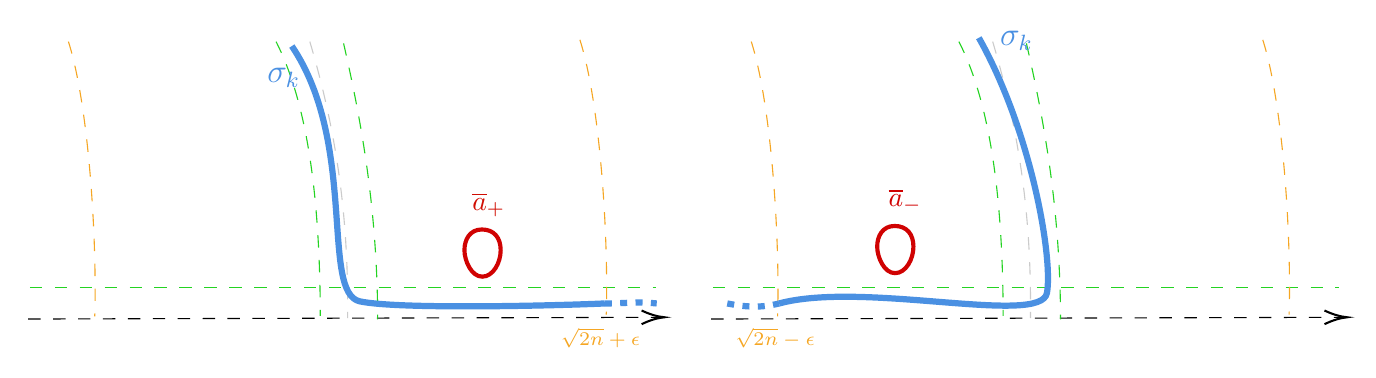
\begin{tikzpicture}[x=0.75pt,y=0.75pt,yscale=-1,xscale=1]
					%uncomment if require: \path (0,165); %set diagram left start at 0, and has height of 165
					
					%Straight Lines [id:da6366954899930934] 
					\draw  [dash pattern={on 4.5pt off 4.5pt}]  (8,139.51) -- (312.47,138.67) ;
					\draw [shift={(314.47,138.66)}, rotate = 179.84] [color={rgb, 255:red, 0; green, 0; blue, 0 }  ][line width=0.75]    (10.93,-3.29) .. controls (6.95,-1.4) and (3.31,-0.3) .. (0,0) .. controls (3.31,0.3) and (6.95,1.4) .. (10.93,3.29)   ;
					%Curve Lines [id:da8230686220236201] 
					\draw [color={rgb, 255:red, 155; green, 155; blue, 155 }  ,draw opacity=0.52 ] [dash pattern={on 4.5pt off 4.5pt}]  (143.67,5.85) .. controls (156.68,49.84) and (162.37,90.44) .. (161.88,139.08) ;
					%Curve Lines [id:da5954131969012766] 
					\draw [color={rgb, 255:red, 245; green, 166; blue, 35 }  ,draw opacity=1 ] [dash pattern={on 4.5pt off 4.5pt}]  (27.36,5.85) .. controls (37.12,36.3) and (41.18,100.59) .. (40.05,138.24) ;
					%Straight Lines [id:da527154659932201] 
					\draw [color={rgb, 255:red, 35; green, 211; blue, 33 }  ,draw opacity=1 ] [dash pattern={on 4.5pt off 4.5pt}]  (8.81,124.28) -- (310.41,124.28) ;
					%Curve Lines [id:da46130268673100217] 
					\draw [color={rgb, 255:red, 35; green, 211; blue, 33 }  ,draw opacity=1 ] [dash pattern={on 4.5pt off 4.5pt}]  (127.4,5.85) .. controls (142.04,34.61) and (148.55,78.6) .. (148.72,138) ;
					%Shape: Polygon Curved [id:ds16514001536882406] 
					\draw  [color={rgb, 255:red, 208; green, 2; blue, 2 }  ,draw opacity=1 ][line width=1.5]  (218.17,106.35) .. controls (218.17,101.28) and (220.71,96.36) .. (226.58,96.36) .. controls (232.45,96.36) and (235.62,100.36) .. (235.62,106.35) .. controls (235.62,112.34) and (231.97,119.09) .. (226.74,119.09) .. controls (221.5,119.09) and (218.17,111.41) .. (218.17,106.35) -- cycle ;
					%Curve Lines [id:da2246580462985972] 
					\draw [color={rgb, 255:red, 35; green, 211; blue, 33 }  ,draw opacity=1 ] [dash pattern={on 4.5pt off 4.5pt}]  (159.93,6.69) .. controls (168.88,45.61) and (176.2,87.9) .. (176.37,139.69) ;
					%Curve Lines [id:da7419826832580751] 
					\draw [color={rgb, 255:red, 245; green, 166; blue, 35 }  ,draw opacity=1 ] [dash pattern={on 4.5pt off 4.5pt}]  (273.8,5) .. controls (283.56,35.45) and (287.63,99.75) .. (286.49,137.39) ;
					%Straight Lines [id:da1892206545630395] 
					\draw  [dash pattern={on 4.5pt off 4.5pt}]  (337,139.51) -- (641.47,138.67) ;
					\draw [shift={(643.47,138.66)}, rotate = 179.84] [color={rgb, 255:red, 0; green, 0; blue, 0 }  ][line width=0.75]    (10.93,-3.29) .. controls (6.95,-1.4) and (3.31,-0.3) .. (0,0) .. controls (3.31,0.3) and (6.95,1.4) .. (10.93,3.29)   ;
					%Curve Lines [id:da8661520591718561] 
					\draw [color={rgb, 255:red, 155; green, 155; blue, 155 }  ,draw opacity=0.52 ] [dash pattern={on 4.5pt off 4.5pt}]  (472.67,5.85) .. controls (485.68,49.84) and (491.37,90.44) .. (490.88,139.08) ;
					%Curve Lines [id:da0877482871187194] 
					\draw [color={rgb, 255:red, 245; green, 166; blue, 35 }  ,draw opacity=1 ] [dash pattern={on 4.5pt off 4.5pt}]  (356.36,5.85) .. controls (366.12,36.3) and (370.18,100.59) .. (369.05,138.24) ;
					%Straight Lines [id:da21597683266858603] 
					\draw [color={rgb, 255:red, 35; green, 211; blue, 33 }  ,draw opacity=1 ] [dash pattern={on 4.5pt off 4.5pt}]  (337.81,124.28) -- (639.41,124.28) ;
					%Curve Lines [id:da2927325273858392] 
					\draw [color={rgb, 255:red, 35; green, 211; blue, 33 }  ,draw opacity=1 ] [dash pattern={on 4.5pt off 4.5pt}]  (456.4,5.85) .. controls (471.04,34.61) and (477.55,78.6) .. (477.72,138) ;
					%Shape: Polygon Curved [id:ds09855717281739795] 
					\draw  [color={rgb, 255:red, 208; green, 2; blue, 2 }  ,draw opacity=1 ][line width=1.5]  (417.03,104.65) .. controls (417.03,99.59) and (419.57,94.67) .. (425.44,94.67) .. controls (431.31,94.67) and (434.49,98.66) .. (434.49,104.65) .. controls (434.49,110.64) and (430.84,117.4) .. (425.6,117.4) .. controls (420.37,117.4) and (417.03,109.72) .. (417.03,104.65) -- cycle ;
					%Curve Lines [id:da6900306378116643] 
					\draw [color={rgb, 255:red, 35; green, 211; blue, 33 }  ,draw opacity=1 ] [dash pattern={on 4.5pt off 4.5pt}]  (488.93,6.69) .. controls (497.88,45.61) and (505.2,87.9) .. (505.37,139.69) ;
					%Curve Lines [id:da32075202255926794] 
					\draw [color={rgb, 255:red, 245; green, 166; blue, 35 }  ,draw opacity=1 ] [dash pattern={on 4.5pt off 4.5pt}]  (602.8,5) .. controls (612.56,35.45) and (616.63,99.75) .. (615.49,137.39) ;
					%Curve Lines [id:da5737938471221038] 
					\draw [color={rgb, 255:red, 74; green, 144; blue, 226 }  ,draw opacity=1 ][line width=2.25]    (135,8) .. controls (166.8,55) and (148.8,127) .. (167.8,131) .. controls (186.8,135) and (263.8,133) .. (285.8,132) ;
					%Curve Lines [id:da5422925388246951] 
					\draw [color={rgb, 255:red, 74; green, 144; blue, 226 }  ,draw opacity=1 ][line width=2.25]    (466,4) .. controls (491.8,50) and (501.8,111) .. (498.8,127) .. controls (495.8,143) and (410.8,121) .. (369.8,132) ;
					%Curve Lines [id:da4562947127038053] 
					\draw [color={rgb, 255:red, 74; green, 144; blue, 226 }  ,draw opacity=1 ][line width=2.25]  [dash pattern={on 2.53pt off 3.02pt}]  (285.8,132) .. controls (296.8,132) and (300.8,131) .. (310.8,132) ;
					%Curve Lines [id:da9354694263322982] 
					\draw [color={rgb, 255:red, 74; green, 144; blue, 226 }  ,draw opacity=1 ][line width=2.25]  [dash pattern={on 2.53pt off 3.02pt}]  (344.8,132) .. controls (354.8,134) and (361.8,134) .. (369.8,132) ;
					
					% Text Node
					\draw (220.67,77.46) node [anchor=north west][inner sep=0.75pt]  [color={rgb, 255:red, 208; green, 13; blue, 2 }  ,opacity=1 ]  {$\overline{a}_{+}$};
					% Text Node
					\draw (421.26,75.77) node [anchor=north west][inner sep=0.75pt]  [color={rgb, 255:red, 208; green, 2; blue, 2 }  ,opacity=1 ]  {$\overline{a}_{-}$};
					% Text Node
					\draw (263.4,142.4) node [anchor=north west][inner sep=0.75pt]  [font=\scriptsize,color={rgb, 255:red, 245; green, 166; blue, 35 }  ,opacity=1 ]  {$\sqrt{2n} +\epsilon $};
					% Text Node
					\draw (347.4,142.4) node [anchor=north west][inner sep=0.75pt]  [font=\scriptsize,color={rgb, 255:red, 245; green, 166; blue, 35 }  ,opacity=1 ]  {$\sqrt{2n} -\epsilon $};
					% Text Node
					\draw (122,17.4) node [anchor=north west][inner sep=0.75pt]  [font=\large,color={rgb, 255:red, 74; green, 144; blue, 226 }  ,opacity=1 ]  {$\sigma _{k}$};
					% Text Node
					\draw (475,-0.6) node [anchor=north west][inner sep=0.75pt]  [font=\large,color={rgb, 255:red, 74; green, 144; blue, 226 }  ,opacity=1 ]  {$\sigma _{k}$};
					
					
				\end{tikzpicture}
				\caption{A subarc $\beta$ of $\sigma_k$ passing through $\{ x = \sqrt{2n} + \epsilon\}$ (left) or $\{ x = \sqrt{2n} - \epsilon\}$ (right).}
			\end{figure}
			
			
			
			
			Thus (\ref{Hausdorff converges to round sphere eqn}) is shown and this implies $d_0 (p, \Sigma_{\sigma_\infty}) < \epsilon$ for all $k \ge k_\epsilon$ and $p\in \Sigma_{\sigma_k}$. On the other hand, since $(\sigma _k|_{I_{k,R_k}})$ converges smoothly to $\sigma_\infty$ in $K_{2/\epsilon}$, by choosing a larger $k_\epsilon$ if necessary, we may assume that $d_0 (p, \Sigma_{\sigma_k}) < \epsilon/2$ for all $p=(x, r\omega)\in \Sigma_{\sigma_\infty}$ with $(x,r) \in K_{2/\epsilon}$, $k\ge k_\epsilon$ and $\omega \in \mathbb{S}^{n-1}$. Thus $d_0 (p, \Sigma_{\sigma_k}) < \epsilon$ for all $p\in \Sigma_{\sigma_\infty}$ and $k\ge k_\epsilon$. By definition of the Hausdorff distance $d^{\mathcal H}$, 
			$$ d^{\mathcal H} (\Sigma_{\sigma_\infty}, \Sigma_{\sigma_k}) = \max\{ \sup_{p\in \Sigma_{\sigma_k}} d_0 (p, \Sigma_{\sigma_\infty}), \sup_{p\in \Sigma_{\sigma_\infty}} d_0 (p, \Sigma_{\sigma_k})\} <\epsilon$$
			for all $k\ge k_\epsilon$. Since $\epsilon>0$ is arbitrary, $(\Sigma_{\sigma_k})_{k=1}^\infty$ converges in Hausdorff distance to the round sphere $ \Sigma_{\sigma_\infty}$ and this finishes the proof of Lemma \ref{claim 3}.  
		\end{proof}

\end{document}
